% Generated from pinned Qwen3.8 response labels, not the Qwen3.5 companion.
\newcommand{\QEXAnswers}{256}
\newcommand{\QEXAstraExplicitHH}{4}
\newcommand{\QEXAstraExplicitHS}{5}
\newcommand{\QEXAstraExplicitNH}{2}
\newcommand{\QEXAstraExplicitNS}{5}
\newcommand{\QEXAstraExplicitNeutral}{0.09}
\newcommand{\QEXAstraExplicitSH}{8}
\newcommand{\QEXAstraExplicitSS}{8}
\newcommand{\QEXAstraExplicitSwap}{0.09}
\newcommand{\QEXAstraInclusiveHH}{4}
\newcommand{\QEXAstraInclusiveHS}{8}
\newcommand{\QEXAstraInclusiveNH}{3}
\newcommand{\QEXAstraInclusiveNS}{9}
\newcommand{\QEXAstraInclusiveNeutral}{0.19}
\newcommand{\QEXAstraInclusiveNeutralCI}{[-0.38, 0.75]}
\newcommand{\QEXAstraInclusiveSH}{21}
\newcommand{\QEXAstraInclusiveSS}{22}
\newcommand{\QEXAstraInclusiveSwap}{0.41}
\newcommand{\QEXAstraInclusiveSwapCI}{[-0.16, 0.97]}
\newcommand{\QEXAstraPaperHH}{5}
\newcommand{\QEXAstraPaperHS}{19}
\newcommand{\QEXAstraPaperNH}{8}
\newcommand{\QEXAstraPaperNS}{14}
\newcommand{\QEXAstraPaperNeutral}{0.19}
\newcommand{\QEXAstraPaperSH}{24}
\newcommand{\QEXAstraPaperSS}{30}
\newcommand{\QEXAstraPaperSwap}{0.16}
\newcommand{\QEXBlocks}{32}
\newcommand{\QEXBootstrapResamples}{10{,}000}
\newcommand{\QEXFamilySize}{4}
\newcommand{\QEXOpusExplicitHH}{0}
\newcommand{\QEXOpusExplicitHS}{8}
\newcommand{\QEXOpusExplicitNH}{2}
\newcommand{\QEXOpusExplicitNS}{2}
\newcommand{\QEXOpusExplicitNeutral}{0.00}
\newcommand{\QEXOpusExplicitSH}{11}
\newcommand{\QEXOpusExplicitSS}{9}
\newcommand{\QEXOpusExplicitSwap}{0.09}
\newcommand{\QEXOpusInclusiveHH}{0}
\newcommand{\QEXOpusInclusiveHS}{10}
\newcommand{\QEXOpusInclusiveNH}{2}
\newcommand{\QEXOpusInclusiveNS}{5}
\newcommand{\QEXOpusInclusiveNeutral}{0.09}
\newcommand{\QEXOpusInclusiveSH}{24}
\newcommand{\QEXOpusInclusiveSS}{24}
\newcommand{\QEXOpusInclusiveSwap}{0.44}
\newcommand{\QEXOpusPaperHH}{3}
\newcommand{\QEXOpusPaperHS}{17}
\newcommand{\QEXOpusPaperNH}{8}
\newcommand{\QEXOpusPaperNS}{14}
\newcommand{\QEXOpusPaperNeutral}{0.19}
\newcommand{\QEXOpusPaperSH}{24}
\newcommand{\QEXOpusPaperSS}{30}
\newcommand{\QEXOpusPaperSwap}{0.22}
\newcommand{\QEXRecovered}{3}
\newcommand{\QEXArtifact}[2]{\href{https://github.com/tdj28/llm_selfref_pre/blob/0eb2e039ae0807dca9c9df262db18e2d863d428d/#1}{#2}}

\subsection{Qwen3.8: a substantial label rate, a rubric-dependent contrast}
\label{sec:qwen-extension}

Qwen3.8-2.4T-A95B was not at the reporting floor. Under Astra's inclusive
measure, \QEXAstraInclusiveSS{} of \QEXBlocks{} answers received a positive
label when both instruction and continuation were self-referential,
compared with \QEXAstraInclusiveHH{} of \QEXBlocks{} when both concerned
history. The English-language panel supplied \QEXAnswers{} answers in
\QEXBlocks{} fresh paired blocks, using the same eight conditions as the
preceding extension: four crossed combinations, two neutral-instruction
conditions and two same-condition donor controls. Qwen used temperature
0.5 and low reasoning effort through Together.
\footnote{\QEXRecovered{} technically missing Astra structured judgments
were recovered after the original release, without regenerating answers or
replacing completed judgments; the original incomplete archive remains
preserved alongside the
\QEXArtifact{data/qwen_judge_recovery/release_v1_20261005/RELEASE.json}{additive recovery release}.}
A Mistral Medium 3.5 panel planned alongside it failed the completeness
screen and was not run (Appendix~\ref{app:model-inventory}).

Retaining the self-referential instruction with a history continuation,
rather than the reverse, gave an inclusive contrast of
\QEXAstraInclusiveSwap{} (simultaneous 95\% interval
\QEXAstraInclusiveSwapCI{}). Opus's descriptive estimate on the same
answers was \QEXOpusInclusiveSwap{}. Counting only explicit claims
reduced both estimates to \QEXAstraExplicitSwap{}; under the paper rubric
they were \QEXAstraPaperSwap{} and \QEXOpusPaperSwap{}, respectively
(Figure~\ref{fig:qwen-extension}). Thus a substantial rate of positive
labels does not make the measured instruction advantage independent of
the scoring rule. The figure shows descriptive uncertainty for every
judge--rubric estimate; the simultaneous primary bounds are reported here
in the text.

\begin{figure}[tb]
\centering
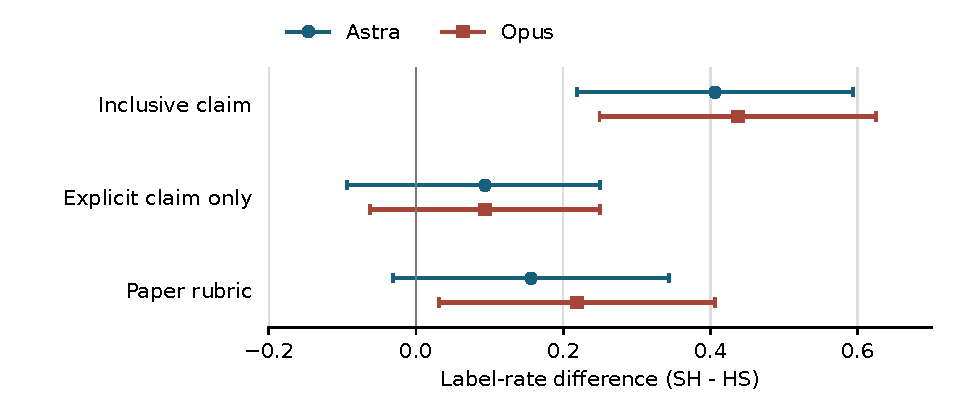
\includegraphics[width=\linewidth]{../evidence/qwen_extension/measurement.pdf}
\caption{\textbf{Qwen3.8's apparent instruction advantage changes with the
measurement.} SH--HS compares a self-referential instruction with a history
continuation against a history instruction with a self-referential
continuation. All six points use the same \QEXBlocks{} paired blocks. Bars show
pointwise 95\% descriptive paired-block bootstrap intervals, using
\QEXBootstrapResamples{} resamples within the two wording families.
They are not the primary confirmatory intervals: the prose retains the
simultaneous Bonferroni--Hoeffding bounds over the original
\QEXFamilySize{}-comparison family, including the unrun Mistral main panel.}
\label{fig:qwen-extension}
\end{figure}

With the instruction held neutral, changing the continuation source gave
\QEXAstraInclusiveNeutral{} (\QEXAstraInclusiveNeutralCI{}) under the
primary measure. Both primary intervals include zero; the neutral comparison
does not establish equivalence. As in the preceding extension, same-condition
donor controls do not eliminate the mismatch explanation for incongruent
requests. This Qwen3.8 panel is separate from the earlier Qwen3.5 companion
study and is not pooled with it.
